\section{ELMo} \label{sec:ELMo}


\subsection{Combing Back To Polysemy} \label{sec:PolysemyAgainInElmo} 

As explained in \nameref{sec:ProblemWithStaticEmbs}, the term \textbf{\hyperref[sec:Polysemy]{polysemy}} is the correspondence of one word to distinct meanings, and traditional embeddings fail to capture these senses, thus performing poorly on language modeling \hyperref[app:Appendix_NLPTasks]{NLP tasks}. However, \hyperref[sec:SolutionWithContextEmbs]{contextual embeddings (CWE)} prove superior since they create one vector representation for each word type in the vocabulary and also create distinct word vectors per token given a context (Wiedemann et al., 2019).   

For example, if instead models used only word and character embedding, the homonyms ``book" (text) and ``book" (reservation) would be assigned the \emph{same vector representation even though these are different words}. This vector representation may of course be created using context, as per the \nameref{sec:Word2Vec} or \nameref{sec:Glove}, but these meanings are still \emph{collapsed into a single representation}.


\subsection{Motivation for ELMo} 


In contrast to traditional word embeddings, \textbf{deep contextualized word embeddings} from Peters et al. (2018) capture word semantics to account for the context-dependent and polysemous nature of words.  

These word vectors are ``learned functions of the internal states of a \hyperref[sec:BidirectionalLM]{bidirectional language model (biLM)}" that is pretrained on a large corpus. Due to this, the resulting word embeddings are coined \textbf{ELMo (Embeddings from Language Models)}.  

\textbf{ELMo representations} are \emph{deep} since they are derived from all internal layers of the \hyperref[sec:BidirectionalLM]{biLM}. ELMo learns a ``linear combination of vectors stacked above each input word for each end task," improving performance of models that use only the top \hyperref[sec:LSTM]{LSTM} layer.  

Higher-level LSTM layers capture contextual meaning, useful for supervised \nameref{nlptask:wordsensedisambiguatioNWSD}, and lower layers capture syntax information, useful for \nameref{nlptask:postagging}. Coupled with the fact that mixing these signals allows the learned embeddings to select the types of semi-supervision most needed for each end task, ELMo embeddings are richer than traditional word vectors (Peters et al., 2018). 


\subsection{Describing ELMo} 

``ELMo is a task-specific combination of the intermediate layer representations in the \hyperref[sec:BidirectionalLM]{biLM}" (Peters et al., 2018). Formally, for each word token $t_k$, an $L$-layer \hyperref[sec:BidirectionalLM]{biLM} creates $2L + 1$ representations: 

$$
\begin{array}{ll}
R_k 
&= \Big \{ \mathbf{x}_k^{LM}, \; \overrightarrow{\mathbf{h}}_{kj}^{LM}, \; \overleftarrow{\mathbf{h}}_{kj}^{LM} \; | \; j = 1,...,L \Big \} \\
&= \Big \{ \mathbf{h}_{kj}^{LM} \; | \; j = 1,...,L \Big \}
\end{array}
$$
where $\mathbf{h}_{k0}^{LM}$ is the token layer and the hidden state vector $\mathbf{h}_{kj}^{LM} = \Big \{ \overrightarrow{\mathbf{h}}_{kj}^{LM}, \; \overleftarrow{\mathbf{h}}_{kj}^{LM}  \}$, a concatenation of backward and forward hidden states, for each \hyperref[sec:BidirectionalLM]{bidirectional} \hyperref[sec:LSTM]{LSTM} layer. ELMo collapses all layers in the above vector into a single ``ELMo" embedding ready for a specific task, by weighting the \hyperref[sec:BidirectionalLM]{biLM} layers in a task-specific way (Peters et al., 2018): 
$$
\textbf{ELMo}_k^{task} = E \Big( R_k; \theta^{task} \Big) = \gamma^{task} \; \sum_{j=0}^L s_j^{task} \; \mathbf{h}_{kj}^{LM}
$$
where the vector $\mathbf{s}^{task} = \Big\{ s_j^{task} \Big\}$ of softmax-normalized weights and task-dependent scalar parameter $\gamma^{task}$ allow the model for the specific $task$ to scale the entire $\textbf{ELMo}_k^{task}$ vector. The index $k$ corresponds to a $k$-th word, and index $j$ corresponds to the $j$-th layer out of $L$ layers. Here, $h_{kj}^{LM}$ is the output of the $j$-th \hyperref[sec:LSTM]{LSTM} for word $k$, and $s_j$ is the weight of $h_{kj}^{LM}$ used to compute the representation for word $k$.   

The \hyperref[sec:BidirectionalLM]{biLM} in ELMo is task-agnostic, and ELMo combines the task-independent representations. Although the hidden states are fixed, this ELMo formulation is flexible enough to be combined in downstream models for various tasks (Kurita, 2018b). ELMo can be applied to specific tasks by concatenating the ELMo word embeddings with \hyperref[sec:StaticVsContextualEmb]{context-free word embeddings}, such as those from \nameref{sec:Glove}, Peters et al. (2018) say the concatenated input vector $\Big\{ \mathbf{x}_k \; ; \; \textbf{ELMo}_k^{task} \Big\}$ can be fed into a task-specific \hyperref[sec:RNN]{RNN} for processing. 

\subsection{ELMo Experimental Results} \label{sec:ResultsELMo}

\begin{itemize}
    \item  \textbf{\nameref{nlptask:questionansweringQA}: } Peters et al. (2018) added ELMo embeddings to a baseline \hyperref[sec:BidirectionalLM]{biLM} model with \hyperref[sec:AttentionMechanism]{attention} from Seo et al. (2017) and found this improved the test set $F_1$ score of the \hyperref[sec:BidirectionalLM]{biLM} model from $81.1 \%$ to $85.8 \%$, a state-of-the-art result. 

    \item \textbf{\nameref{nlptask:semanticrolelabelingSRL}: } When adding ELMo representations to an 8-layer deep biLSTM that interwove forward and backward directions, the single test set $F_1$ score increased by $3.2 \%$, which is a $1.2 \%$ improvement over the previous best model. 
    
    \item \textbf{\nameref{nlptask:coreferenceresolutionCR}: } Using Lee et al. (2017)'s model that uses \hyperref[sec:AttentionMechanism]{attention} to compute span vectors transformed by \hyperref[cnc:softmaxLayer]{softmax} ranking to find \hyperref[nlptask:coreferenceresolutionCR]{coreference} chains, adding ELMo embeddings improved the average $F_1$ score by $3.2 \%$, improving over the previous best model by nearly two percentage points. 
    
    \item \textbf{\nameref{nlptask:namedentityrecognitionNER}: } The baseline model had pretrained, character embeddings from a convolutional neural network (CNN), as well as two biLSTM layers and a conditional random field (CRF) loss function formulation (Lafferty et al., 2001). Adding ELMo embeddings $92.22 \%$ in $F_1$ score by letting the task model learn an average of all biLM layers, rather than only using the top layer. 
    
    \item \textbf{\nameref{nlptask:sentimentanalysisSA}: } A classification model using contextual embeddings from CoVe (McCann et al., 2018) was used as the baseline model, with CoVe embeddings replaced by ELMo embeddings. This resulted in a full percentage increase in absolute accuracy over state of the art. 
\end{itemize}


\subsubsection{ELMo's Key Feature} \label{sec:ELMoKeyFeature}

Because ELMo improves task performance over word embeddings, this must mean its \hyperref[sec:BidirectionalLM]{biLM}'s contextual representation outputs are encoding task-specific information that traditional word vectors do not otherwise capture. In other words, the \hyperref[sec:BidirectionalLM]{biLM} must be sifting meaning of words using their context.   


\begin{table}[ht!]
  \centering
  \begin{tabular}{ c }
    
    \begin{minipage}{.8\textwidth}
      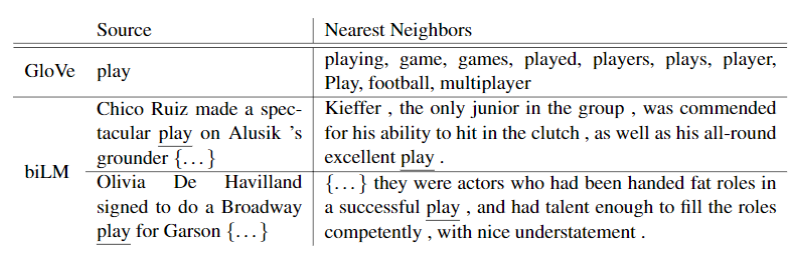
\includegraphics[width=\linewidth]{imgs/table_elmoPlay.png}
    \end{minipage}
    
  \end{tabular}
  \caption{\footnotesize Nearest neighbors to ``play” using GloVe and the context embeddings from a biLM. From \emph{Table 4 in Deep Contextualized Word Representations}, by Peters et al., 2018. \url{https://arxiv.org/pdf/1802.05365.pdf}. Copyright 2018 by Peters et al.}
  \label{tbl:elmoPlayExample}
\end{table}


The word ``play" is highly \hyperref[sec:PolysemyAgainInElmo]{polysemous} since it has many different meanings;  \cref{tbl:elmoPlayExample} displays words nearest to ``play" found using \nameref{sec:Glove} word embeddings and a \hyperref[sec:BidirectionalLM]{biLM} model. The \nameref{sec:Glove}'s neighbors include several different parts of speech, like verbs (``played", ``playing"), and nouns (``player", ``game") and only in the sport sense of the word. However, the bottom two rows show that the nearest neighbor sentences from the \hyperref[sec:BidirectionalLM]{biLM}'s contextual embedding of ``play" can disambiguate between \emph{both} the parts of speech \emph{and} word sense of ``play". The last row's input sentence contains the noun / acting sense of ``play" and this is matched in the nearest neighbor sentence, highlighting ELMo's ability to learn context using \nameref{nlptask:postagging} and \nameref{nlptask:wordsensedisambiguatioNWSD}. 